%\document class[]{aiaa-tc} %load in aiaa class template file
\documentclass{article}
\usepackage{amsmath}
\usepackage{mathrsfs}
\usepackage{enumitem}
\usepackage{mathabx}
\usepackage{hyperref}
\usepackage{natbib} %REMOVE THIS IF YOU DON'T WANT BRACKETS ON YOUR PAPER
\usepackage{float}
\usepackage{color,soul}
\usepackage[font=normalsize,labelfont=bf]{caption}
\usepackage[left=2cm,right=2cm,top=2cm,bottom=2cm]{geometry}
\usepackage{graphicx}

\newcommand{\sref}[1]{$^{[\ref{#1}]}$}
\newcommand{\dref}[2]{$^{[\ref{#1}-\ref{#2}]}$}

 % Define commands to assure consistent treatment throughout document
\newcommand{\eqnref}[1]{(\ref{#1})}
\newcommand{\class}[1]{\texttt{#1}}
\newcommand{\package}[1]{\texttt{#1}}
\newcommand{\file}[1]{\texttt{#1}}
\newcommand{\BibTeX}{\textsc{Bib}\TeX}

\begin{document}

\begin{center}
\begin{LARGE}{\bf Project Based Engineering Instrumentation With CircuitPython}\end{LARGE}\\
\large
\vspace{22 mm}
   A Brief Textbook Presented to the \\ 
   Student Body of the University of South Alabama \\
\vspace{22 mm}
%%by\\
\vspace{22 mm}
  %%Carlos Montalvo \\
\vspace{22 mm}
       %%{\itshape University of South Alabama}\\
       Last Update: \today\\
{\bf Copyright $\copyright$ Carlos Jos\'{e} Montalvo}
\end{center}

\linespread{1}

\newpage

\noindent This textbook has been purchased by Tangibles that Teach and as such
has moved to the following url\\
\url{https://a2279211-28c1-4f46-9477-0d3265900c7f.filesusr.com/ugd/2413aa_97652967fb374bb38aa9f9906739ef9c.pdf}
\ \\
The kit used in this textbook can be purchased here\\
\url{https://www.tangiblesthatteach.com/product-page/instrumentation-kit-for-me-316}.
\ \\
A preview of the textbook has been included but only the first few
chapters as an example.

\newpage

\section*{Acknowledgements}

The author, Dr. Carlos Montalvo would like to acknowledge a few key
members who made this textbook possible. First and foremost I would
like to thank Adafruit for their entire ecosystem of electronics,
tutorials, blogs and forums. Much of what I have learned here to teach
Instrumentation was from \href{https://www.adafruit.com/}{Adafruit}
and the \href{https://learn.adafruit.com/}{Adafruit Learn} system and 
specifically people like Lady Ada and John Park who have helped shape
\href{https://circuitpython.org/}{CircuitPython} and the
\href{https://www.adafruit.com/product/3333}{CircuitPlayground
  Express} to what it is today. I 
would also like to thank Dr. Saami Yazdani for creating the blueprint
for Instrumentation at my university by creating a laboratory
environment for an otherwise totally theoretical course. His course
was the foundation for this textbook and for that I thank him for
showing the way. I’d like to also thank and acknowledge Tangibles that
Teach for giving me the opportunity to morph this loose set of
projects into a textbook that can be used for multiple universities
and classrooms and of course help students learn and acquire knowledge
through creating.

\section*{About this textbook}

This textbook has been designed with the student and faculty member in
mind. First, this textbook goes hand in hand with Engineering
Instrumentation taught at the undergraduate level at many
universities. The course begins with simple plotting and moves into
data analysis, calibration and more complex instrumentation techniques
such as active filtering and aliasing. This course is designed to get
students away from their pen and paper and build something that blinks
and moves as well as learn to process real data that they themselves
acquire. There is no theory in these projects. It is all applied using
the project based learning method. Students will be tasked with
downloading code, building circuitry, taking data all from the ground
up. By the end of this course students will be well versed in the
desktop version of Python while also the variant CircuitPython
designed specifically for microelectronics from Adafruit. After this
course students will be able to understand Instrumentation at the
fundamental level as well as generate code that can be used in future
projects and research to take and analyze data. Python is such a broad
and useful language that it will be very beneficial for any
undergraduate student to learn this language. To the professors using
this textbook, 1 credit hour labs are often hard to work into a
curriculum and “live” demonstrations in the classroom cost time and
money that take away from other faculty duties. I’ve created this kit
and textbook to be completely stand-alone. Students simply need to
purchase the required materials and follow along with the
lessons. These lessons can be picked apart and taught sequentially or
individually on a schedule suited to the learning speed of the
course. I hope whomever reads and learns from this textbook will walk
away with an excitement to tinker, code and build future projects
using microelectronics and programming.

\newpage

\tableofcontents

\newpage

\section{Purchase Instrumentation Equipment}

In this class you’re going to build some circuits that will enhance
your learning experience. Rather than just solving problems by hand
you’re going to take and analyze data. Over the summer of 2020, I
wrote a textbook with
\href{https://www.tangiblesthatteach.com/shop}{Tangibles that Teach}
and they have graciously 
bundled all components together. The price is \$50 plus shipping so
it’s about the same price as below but you’ll probably save on
shipping from multiple vendors and everything is all in one place
which is nice. There is an
\href{https://www.tangiblesthatteach.com/downloads}{accompanying textbook that can be downloaded} as well. 

When you get your kit familiarize yourself with all of the
components. I created an
\href{https://youtu.be/6sNNQrhnzLE}{unboxing video on Youtube} for you
to take a look. Below is also a photo of all the components.
\begin{figure}[H]
  \begin{center}
    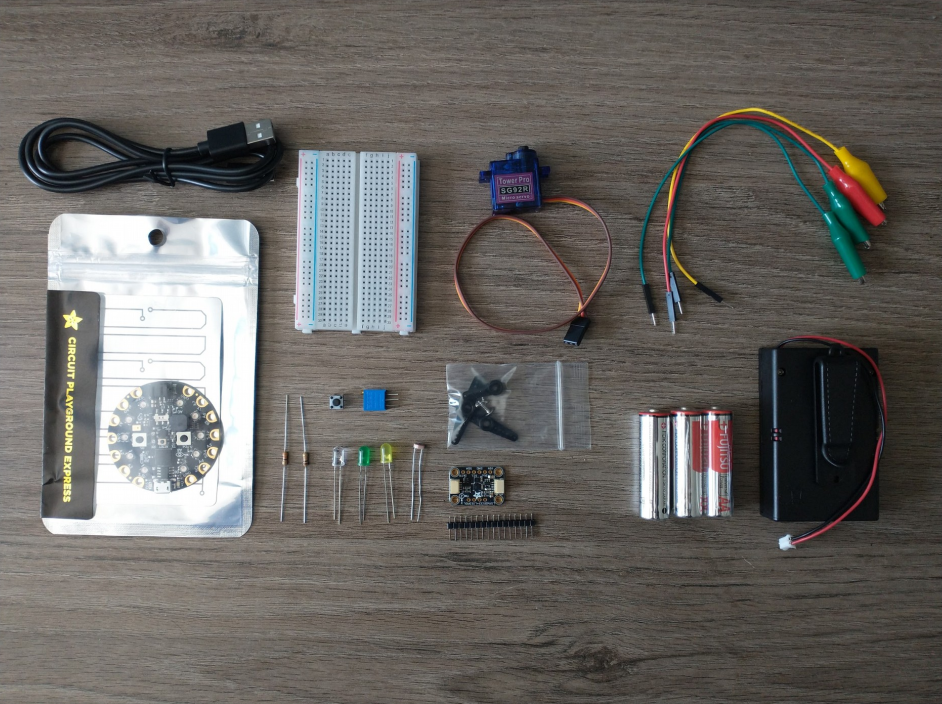
\includegraphics[width=\textwidth]{Figures/components.png}
  \end{center}
\end{figure}

\subsection{Quick Links}

\begin{enumerate}[itemsep=-5pt]
  \item \href{https://www.tangiblesthatteach.com/product-page/instrumentation-kit-for-me-316}{Kit}
  \item \href{https://a2279211-28c1-4f46-9477-0d3265900c7f.filesusr.com/ugd/2413aa_ca39175b0a514b838ec96893b90590eb.pdf}{Document}
  \item \href{https://youtu.be/6sNNQrhnzLE}{Unboxing Video}
\end{enumerate}

\subsection{Turning in this assignment}

\begin{enumerate}[itemsep=-5pt]
  \item Upload a receipt of ALL of your purchases - 50\%
  \item Put your name and the names of your group members. If working
    alone, tell me you are planning on working alone in the PDF you
    upload. In times of COVID, everyone is working alone - 50\%
\end{enumerate}

\newpage

\begin{center}\LARGE{ONLY READ BELOW IF YOU DON’T WANT TO BUY THE KIT
    ABOVE}\end{center}

\subsection{Purchase Items Yourself}

The bill of materials listed below is designed for 2 or 4 students to work together and share
pieces. This kit is not optimized for 3 students. If you are a remote/online student or you just
prefer to work alone then you have the option of purchasing everything yourself. The cost per
student in a group of 4 and 2 is listed as well as the cost if working alone. You’ll find that even
with the optional equipment, the cost of working alone is still less than the price of a standard
college textbook. Note that if you are working alone, be sure to only purchase 1 of each item. If
working in pairs you also have the option of purchasing one of each item. Finally, if you own
some of these components you may wish to simply purchase each item separately. A detailed
parts breakdown is shown after the rubric.

\subsection{Bill of Materials (per 4 students)}

\begin{figure}[H]
  \begin{center}
    \begin{tabular}{|l|c|c|}
      \hline
      Item (ONLY IF YOU DON’T WANT THE KIT ABOVE) & Quantity & Total
      Cost \\
      \hline
      \href{https://www.adafruit.com/product/3333}{Circuit Playground Express (CPX)} & 2 & \$50 \\
      \hline
      Servo & 2 & \$10 \\
      \hline
      USB Cable & 2 & \$6 \\
      \hline
      Electronics Kit (Photocells, Resistors, Trimpot) & 1 & \$13 \\
      \hline
      Alligator Clips & 1 & \$4 \\
      \hline
      {\bf Total} & & {\bf \$83} \\
      \hline
      {\bf Cost per student in a group of 4} & & {\bf \$21} \\
      \hline
      {\bf Cost per student in a group of 2} & & {\bf \$25} \\
      \hline
      {\bf Cost if working alone} & & {\bf \$50} \\
      \hline
       & & \\
      \hline
      {\bf Optional Equipment} & & \\
      \hline
      External Power Supply & 2 & \$6 \\
      \hline
      AA Batteries & 2 & \$6 \\
      \hline
      Analog Pitot Probe & 1 & \$31 \\
      \hline
      Rate Gyro (LSM6D3SS) & 1 & \$10 \\
      \hline
      & & \\
      \hline
      {\bf Total with Optional Equipment} & & {\bf \$136} \\
      \hline
      {\bf Cost per student in a group of 4} & & {\bf \$34} \\
      \hline
      {\bf Cost per student in a group of 2} & & {\bf \$50} \\
      \hline
      {\bf Cost if working alone} & & {\bf \$97} \\
      \hline
    \end{tabular}
  \end{center}
\end{figure}



\end{document}
